% questions.tex —— 2003 年·上海卷·理科 · 题目内容片段（无答案）
% 由 tools/generate_projects.py 依来源总账自 2003/2003_数学真题_上海理_试题.md 生成，勿手改（改源 MD 后重跑）


\begin{gktip}
\textbf{来源说明}：本稿依据固定候选 \texttt{src-1c1b7702523f8dab3f1fb274ae6d8c631a291090d33ddb6e3d9f3d8de897a1d0}（SHA-256 \texttt{88b72fea05d331215504bb89257e375d07c18ba21e830cf9e6288461e88ccf8d}）的 PDF 第 1–2 页逐题转录，原卷印刷页码 138–139。来源发布者、版次、复制/扫描链及官方身份未核；该 source 与本库内部 paper 的绑定不代表官方身份认证。固定 PDF 仅含题面，无答案或评分页，\texttt{official_answer} 为 \texttt{null}。
\textbf{图表说明}：Q16、Q18、Q20 依固定原页重绘为 TikZ 示意图；具体坐标和比例不作题设断言。
\textbf{待核保留}：Q14 未明示两平面互异。严格面面平行定义下，题面不能排除两平面重合，答案保留 U/PENDING；若默认平面互异，预期选项为 D。
\end{gktip}

\gkpart{一、填空题}

\begin{question}
\gkti{1}函数
\nopagebreak[4]
\[
   y=\sin x\cos\left(x+\frac{\pi}{4}\right)+\cos x\sin\left(x+\frac{\pi}{4}\right)
\]
   的最小正周期 \(T=\underline{\qquad}\)。

\end{question}
\begin{question}
\gkti{2}若 \(x=\dfrac{\pi}{3}\) 是方程 \(2\cos(x+\alpha)=1\) 的解，其中 \(\alpha\in(0,2\pi)\)，则 \(\alpha=\underline{\qquad}\)。

\end{question}
\begin{question}
\gkti{3}在等差数列 \(\{a_n\}\) 中，\(a_5=3,\ a_6=-2\)，则 \(a_4+a_5+\cdots+a_{10}=\underline{\qquad}\)。

\end{question}
\begin{question}
\gkti{4}在极坐标系中，定点 \(A\left(1,\dfrac{\pi}{2}\right)\)，点 \(B\) 在直线
\nopagebreak[4]
\[
   \rho\cos\theta+\rho\sin\theta=0
\]
   上运动。当线段 \(AB\) 最短时，点 \(B\) 的极坐标是 \(\underline{\qquad}\)。

\end{question}
\begin{question}
\gkti{5}在正四棱锥 \(P-ABCD\) 中，若侧面与底面所成二面角的大小为 \(60^\circ\)，则异面直线 \(PA\) 与 \(BC\) 所成角的大小等于 \(\underline{\qquad}\)。（结果用反三角函数值表示）

\end{question}
\begin{question}
\gkti{6}设集合
\nopagebreak[4]
\[
   A=\{x\mid |x|<4\},\qquad B=\{x\mid x^2-4x+3>0\},
\]
   则集合 \(\{x\mid x\in A\text{ 且 }x\notin A\cap B\}=\underline{\qquad}\)。

\end{question}
\begin{question}
\gkti{7}在 \(\triangle ABC\) 中，\(\sin A:\sin B:\sin C=2:3:4\)，则 \(\angle ABC=\underline{\qquad}\)。（结果用反三角函数值表示）

\end{question}
\begin{question}
\gkti{8}若首项为 \(a_1\)、公比为 \(q\) 的等比数列 \(\{a_n\}\) 的前 \(n\) 项和总小于这个数列的各项和，则首项 \(a_1\)、公比 \(q\) 的一组取值可以是 \((a_1,q)=\underline{\qquad}\)。

\end{question}
\begin{question}
\gkti{9}某国际科研合作项目成员由 11 个美国人、4 个法国人和 5 个中国人组成。现从中随机选出两位作为成果发布人，则此两人不属于同一个国家的概率为 \(\underline{\qquad}\)。（结果用分数表示）

\end{question}
\begin{question}
\gkti{10}方程 \(x^3+\lg x=18\) 的根 \(x\approx\underline{\qquad}\)。（结果精确到 0.1）

\end{question}
\begin{question}
\gkti{11}已知点
\nopagebreak[4]
\[
    A\left(0,\frac{2}{n}\right),\quad B\left(0,-\frac{2}{n}\right),\quad C\left(4+\frac{2}{n},0\right),
\]
\Needspace{5\baselineskip}
    其中 \(n\) 为正整数。设 \(S_n\) 表示 \(\triangle ABC\) 外接圆的面积，则
\nopagebreak[4]
\[
    \lim_{n\to\infty}S_n=\underline{\qquad}\mbox{。}
\]

\end{question}
\begin{question}
\gkti{12}给出问题：\(F_1、F_2\) 是双曲线
\nopagebreak[4]
\[
    \frac{x^2}{16}-\frac{y^2}{20}=1
\]
\Needspace{5\baselineskip}
    的焦点，点 \(P\) 在双曲线上。若点 \(P\) 到焦点 \(F_1\) 的距离等于 9，求点 \(P\) 到焦点 \(F_2\) 的距离。某学生的解答如下：双曲线的实轴长为 8，由
\nopagebreak[4]
\[
    \bigl||PF_1|-|PF_2|\bigr|=8,
\]
    即 \(|9-|PF_2||=8\)，得 \(|PF_2|=1\) 或 17。该学生的解答是否正确？若正确，请将他的解题依据填在下面空格内；若不正确，将正确的结果填在下面空格内 \(\underline{\qquad}\)。

\end{question}
\gkpart{二、选择题}

\begin{question}
\gkti{13}下列函数中，既为偶函数又在 \((0,\pi)\) 上单调递增的是\mbox{（　　）}

    (A) \(y=\tan|x|\)　　(B) \(y=\cos(-x)\)

    (C) \(y=\sin\left(x-\dfrac{\pi}{2}\right)\)　　(D) \(y=\left|\cot\dfrac{x}{2}\right|\)

\end{question}
\begin{question}
\gkti{14}在下列条件中，可判断平面 \(\alpha\) 与 \(\beta\) 平行的是\mbox{（　　）}

    (A) \(\alpha、\beta\) 都垂直于平面 \(\gamma\)

    (B) \(\alpha\) 内存在不共线的三点到 \(\beta\) 的距离相等

    (C) \(l,m\) 是 \(\alpha\) 内两条直线，且 \(l\parallel\beta,\ m\parallel\beta\)

    (D) \(l,m\) 是两条异面直线，且 \(l\parallel\alpha,\ m\parallel\alpha,\ l\parallel\beta,\ m\parallel\beta\)

\end{question}
\begin{question}
\gkti{15}\(a_1,b_1,c_1,a_2,b_2,c_2\) 均为非零实数。不等式
\nopagebreak[4]
\[
    a_1x^2+b_1x+c_1>0\quad\text{和}\quad a_2x^2+b_2x+c_2>0
\]
\Needspace{5\baselineskip}
    的解集分别为集合 \(M\) 和 \(N\)，那么
\nopagebreak[4]
\[
    \frac{a_1}{a_2}=\frac{b_1}{b_2}=\frac{c_1}{c_2}
\]
    是“\(M=N\)”的\mbox{（　　）}

    (A) 充分非必要条件　　(B) 必要非充分条件　　(C) 充要条件　　(D) 既非充分又非必要条件

\Needspace{0.4\textheight}
\end{question}
\begin{question}
\gkti{16}\(f(x)\) 是定义在区间 \([-c,c]\) 上的奇函数，其图象如图所示。令 \(g(x)=af(x)+b\)，则下列关于函数 \(g(x)\) 的叙述正确的是\mbox{（　　）}

    (A) 若 \(a<0\)，则函数 \(g(x)\) 的图象关于原点对称

    (B) 若 \(a=-1,\ -2<b<0\)，则方程 \(g(x)=0\) 有大于 2 的实根

    (C) 若 \(a\ne0,\ b=2\)，则方程 \(g(x)=0\) 有两个实根

    (D) 若 \(a\ge1,\ b<2\)，则方程 \(g(x)=0\) 有三个实根
\nopagebreak[4]
\begin{center}% Generator: hand-authored TikZ schematic.
% Source ID: src-1c1b7702523f8dab3f1fb274ae6d8c631a291090d33ddb6e3d9f3d8de897a1d0
% PDF SHA-256: 88b72fea05d331215504bb89257e375d07c18ba21e830cf9e6288461e88ccf8d
% Source location: PDF page 1, printed page 138, Question 16.
\begin{tikzpicture}[>=stealth,line cap=round,line join=round]
  % Schematic coordinates only; the drawing does not assert scale or exact extrema.
  \draw[->] (-3.9,0)--(3.9,0) node[right] {$x$};
  \draw[->] (0,-2.9)--(0,2.9) node[above] {$y$};

  % Odd-shaped curve: nonzero intercepts lie in (-c,-2) and (2,c).
  % The x-axis labels -2 and 2 are not intercepts or extremum abscissae.
  \draw[thick]
    plot[smooth] coordinates {
      (-3.05,2.55) (-2.85,1.7) (-2.55,0) (-2.1,-1.55)
      (-1.5,-2) (-0.8,-1.5) (0,0) (0.8,1.5)
      (1.5,2) (2.1,1.55) (2.55,0) (2.85,-1.7) (3.05,-2.55)
    };
  \node[above left] at (-3.02,2.05) {$y=f(x)$};

  % Dashed guides at x=+-c and y=+-2.
  \draw[dashed] (-3.05,0)--(-3.05,2.55);
  \draw[dashed] (3.05,0)--(3.05,-2.55);
  \draw[dashed] (0,2)--(1.5,2);
  \draw[dashed] (0,-2)--(-1.5,-2);

  \node[left] at (0,2) {$2$};
  \node[left] at (0,-2) {$-2$};
  \node[below left] at (0,0) {$O$};
  \node[below] at (-3.05,0) {$-c$};
  \node[below] at (-2,0) {$-2$};
  \node[below] at (2,0) {$2$};
  \node[below] at (3.05,0) {$c$};
\end{tikzpicture}
\end{center}
\nopagebreak[4]
\end{question}
\gkpart{三、解答题}

\begin{question}
\gkti{17}已知复数 \(z_1=\cos\theta-i,\ z_2=\sin\theta+i\)，求 \(|z_1\cdot z_2|\) 的最大值和最小值。

\Needspace{0.4\textheight}
\end{question}
\begin{question}
\gkti{18}已知平行六面体 \(ABCD-A_1B_1C_1D_1\) 中，\(A_1A\perp\) 平面 \(ABCD\)，\(AB=4,\ AD=2\)。若 \(B_1D\perp BC\)，直线 \(B_1D\) 与平面 \(ABCD\) 所成的角等于 \(30^\circ\)，求平行六面体 \(ABCD-A_1B_1C_1D_1\) 的体积。
\nopagebreak[4]
\begin{center}% Generator: hand-authored TikZ schematic.
% Source ID: src-1c1b7702523f8dab3f1fb274ae6d8c631a291090d33ddb6e3d9f3d8de897a1d0
% PDF SHA-256: 88b72fea05d331215504bb89257e375d07c18ba21e830cf9e6288461e88ccf8d
% Source location: PDF page 1, printed page 138, Question 18.
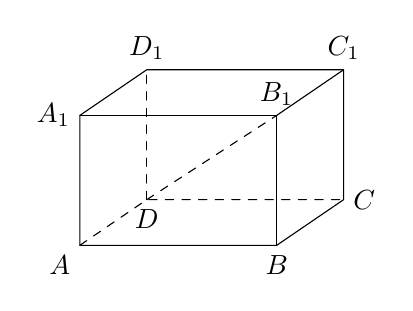
\begin{tikzpicture}[line cap=round,line join=round]
  % Schematic projection only; edge lengths and angles are not asserted.
  \coordinate (A)  at (0,0);
  \coordinate (B)  at (2.5,0);
  \coordinate (C)  at (3.35,0.58);
  \coordinate (D)  at (0.85,0.58);
  \coordinate (A1) at (0,1.65);
  \coordinate (B1) at (2.5,1.65);
  \coordinate (C1) at (3.35,2.23);
  \coordinate (D1) at (0.85,2.23);

  % Solid visible edges.
  \draw (A)--(B)--(C)--(C1)--(D1)--(A1)--(A);
  \draw (A1)--(B1)--(B);
  \draw (B1)--(C1);
  % Hidden edges and the explicitly shown diagonal B1D.
  \draw[dashed] (A)--(D)--(C);
  \draw[dashed] (D)--(D1);
  \draw[dashed] (D)--(B1);

  \node[below left] at (A) {$A$};
  \node[below] at (B) {$B$};
  \node[right] at (C) {$C$};
  \node[below] at (D) {$D$};
  \node[left] at (A1) {$A_1$};
  \node[above] at (B1) {$B_1$};
  \node[above] at (C1) {$C_1$};
  \node[above] at (D1) {$D_1$};
\end{tikzpicture}
\end{center}
\nopagebreak[4]
\end{question}
\begin{question}
\gkti{19}已知数列 \(\{a_n\}\)（\(n\) 为正整数）是首项是 \(a_1\)、公比为 \(q\) 的等比数列。

\Needspace{5\baselineskip}
    (1) 求和：
\nopagebreak[4]
\[
    a_1C_2^0-a_2C_2^1+a_3C_2^2,\qquad
    a_1C_3^0-a_2C_3^1+a_3C_3^2-a_4C_3^3；
\]

    (2) 由 (1) 的结果归纳概括出关于正整数 \(n\) 的一个结论，并加以证明。

\Needspace{0.4\textheight}
\end{question}
\begin{question}
\gkti{20}如图，某隧道设计为双向四车道，车道总宽 22 米，要求通行车辆限高 4.5 米，隧道全长 2.5 千米，隧道的拱线近似地看成半个椭圆形状。

    (1) 若最大拱高 \(h\) 为 6 米，则隧道设计的拱宽 \(l\) 是多少？

    (2) 若最大拱高 \(h\) 不小于 6 米，则应如何设计拱高 \(h\) 和拱宽 \(l\)，才能使半个椭圆形隧道的土方工程量最小？

    注：半个椭圆的面积公式为 \(S=\dfrac{\pi}{4}lh\)，柱体体积为：底面积乘以高。本题结果精确到 0.1 米。
\nopagebreak[4]
\begin{center}% Generator: hand-authored TikZ schematic.
% Source ID: src-1c1b7702523f8dab3f1fb274ae6d8c631a291090d33ddb6e3d9f3d8de897a1d0
% PDF SHA-256: 88b72fea05d331215504bb89257e375d07c18ba21e830cf9e6288461e88ccf8d
% Source location: PDF page 2, printed page 139, Question 20.
\begin{tikzpicture}[x=0.72cm,y=0.72cm,>=stealth,line cap=round,line join=round]
  % Schematic coordinates only; no metric scale or ellipse dimensions are asserted.
  % Upper half-ellipse tunnel arch and ground-level coordinate axes.
  \draw[thick] (-4.4,0) arc[start angle=180,end angle=0,x radius=4.4,y radius=2.2];
  \draw[->] (-5.2,0)--(5.15,0) node[right] {$x$};
  \draw[->] (0,-0.25)--(0,3.05) node[above] {$y$};
  \node[above right] at (2.15,2.75) {（单位：米）};

  % The 4.5 m level and schematic lane-separator dashes.
  \draw[dashed] (-3.12,1.38)--(3.12,1.38);
  \draw[dashed] (-3.12,0)--(-3.12,1.38);
  \draw[dashed] (-1.56,0)--(-1.56,1.38);
  \draw[dashed] (1.56,0)--(1.56,1.38);
  \draw[dashed] (3.12,0)--(3.12,1.38);

  % 4.5 vertical measure, with its source-visible horizontal witness line.
  \draw (-5.75,1.38)--(-3.12,1.38);
  \draw[<->] (-4.82,0.04)--(-4.82,1.34);
  \node[left] at (-4.82,0.69) {$4.5$};

  % Maximum height h from the x-axis to the arch apex, with a top witness
  % line running from the apex to the left side of the height arrow.
  \draw (0,2.2)--(4.55,2.2);
  \draw[<->] (4.55,0.04)--(4.55,2.16);
  \node[right] at (4.55,1.12) {$h$};

  % Roadway width 22 at y=4.5 and full tunnel base width l.
  \draw ( -3.12,0)--(-3.12,-0.62);
  \draw (  3.12,0)--( 3.12,-0.62);
  \draw[<->] (-3.08,-0.54)--(3.08,-0.54);
  \node[fill=white,inner sep=1pt] at (0,-0.54) {$22$};
  \draw (-4.4,0)--(-4.4,-1.28);
  \draw ( 4.4,0)--( 4.4,-1.28);
  \draw[<->] (-4.36,-1.18)--(4.36,-1.18);
  \node[fill=white,inner sep=1pt] at (0,-1.18) {$l$};
\end{tikzpicture}
\end{center}
\nopagebreak[4]
\end{question}
\begin{question}
\gkti{21}在以 \(O\) 为原点的直角坐标系中，点 \(A(4,-3)\) 为 \(\triangle OAB\) 的直角顶点。已知 \(|AB|=2|OA|\)，且点 \(B\) 的纵坐标大于零。

    (1) 求向量 \(\overrightarrow{AB}\) 的坐标；

    (2) 求圆 \(x^2-6x+y^2+2y=0\) 关于直线 \(OB\) 对称的圆的方程；

    (3) 是否存在实数 \(a\)，使抛物线 \(y=ax^2-1\) 上总有关于直线 \(OB\) 对称的两点？若不存在，说明理由；若存在，求 \(a\) 的取值范围。

\end{question}
\begin{question}
\gkti{22}已知集合 \(M\) 是满足下列性质的函数 \(f(x)\) 的全体：存在非零常数 \(T\)，对任意 \(x\in\mathbb{R}\)，有 \(f(x+T)=Tf(x)\) 成立。

    (1) 函数 \(f(x)=x\) 是否属于集合 \(M\)？说明理由；

    (2) 设函数 \(f(x)=a^x\)（\(a>0\)，且 \(a\ne1\)）的图象与 \(y=x\) 的图象有公共点，证明：\(f(x)=a^x\in M\)；

    (3) 若函数 \(f(x)=\sin kx\in M\)，求实数 \(k\) 的取值范围。

\end{question}